\byline{{\textbf{\Large\sffamily February Bonsai Club Meetup:}}\\
        {\textbf{\large\sffamily Love is in the Air\dots and in Our Trees!}}}{The Newsletter Team}

\noindent
Despite a few familiar faces missing, February's meeting saw a high turnout with 21 members, proving our club's enthusiasm is as strong as ever. 

The highlight of the evening was \textbf{Steve's grafting workshop}, where members carefully grafted Paul's Scarlet onto Common Hawthorn.
Now, with fingers crossed, we eagerly await the results!
While some focused on grafting, others worked on their trees, and Adam brought a tree for critique and also surprised members with a \textbf{flash sale}, offering a few bonsai\--related bargains.

Our \textbf{Tree of the Month} and \textbf{Novice Tree of the Month} competitions featured the theme \textit{``Carved, Jin's, Uro's,''} leading to some striking entries that showcased the skill and creativity of our members.  

A special mention goes to our \textbf{Winter Show}, which was a tremendous success.
The new venue allowed for an elevated display, featuring two stunning \textbf{Chelsea Flower Show Gold Medal\--winning trees} and two \textbf{suiseki tables}, a new and welcome addition.
Visitors enjoyed browsing \textbf{vendor stalls}, the ever\--popular \textbf{bargain table}, and a \textbf{tombola}, while the \textbf{workshop area} kept both newcomers and seasoned enthusiasts engaged.

A huge thank you to all who attended---we look forward to seeing everyone again in March!

\begin{window}[%
    2,l,%
    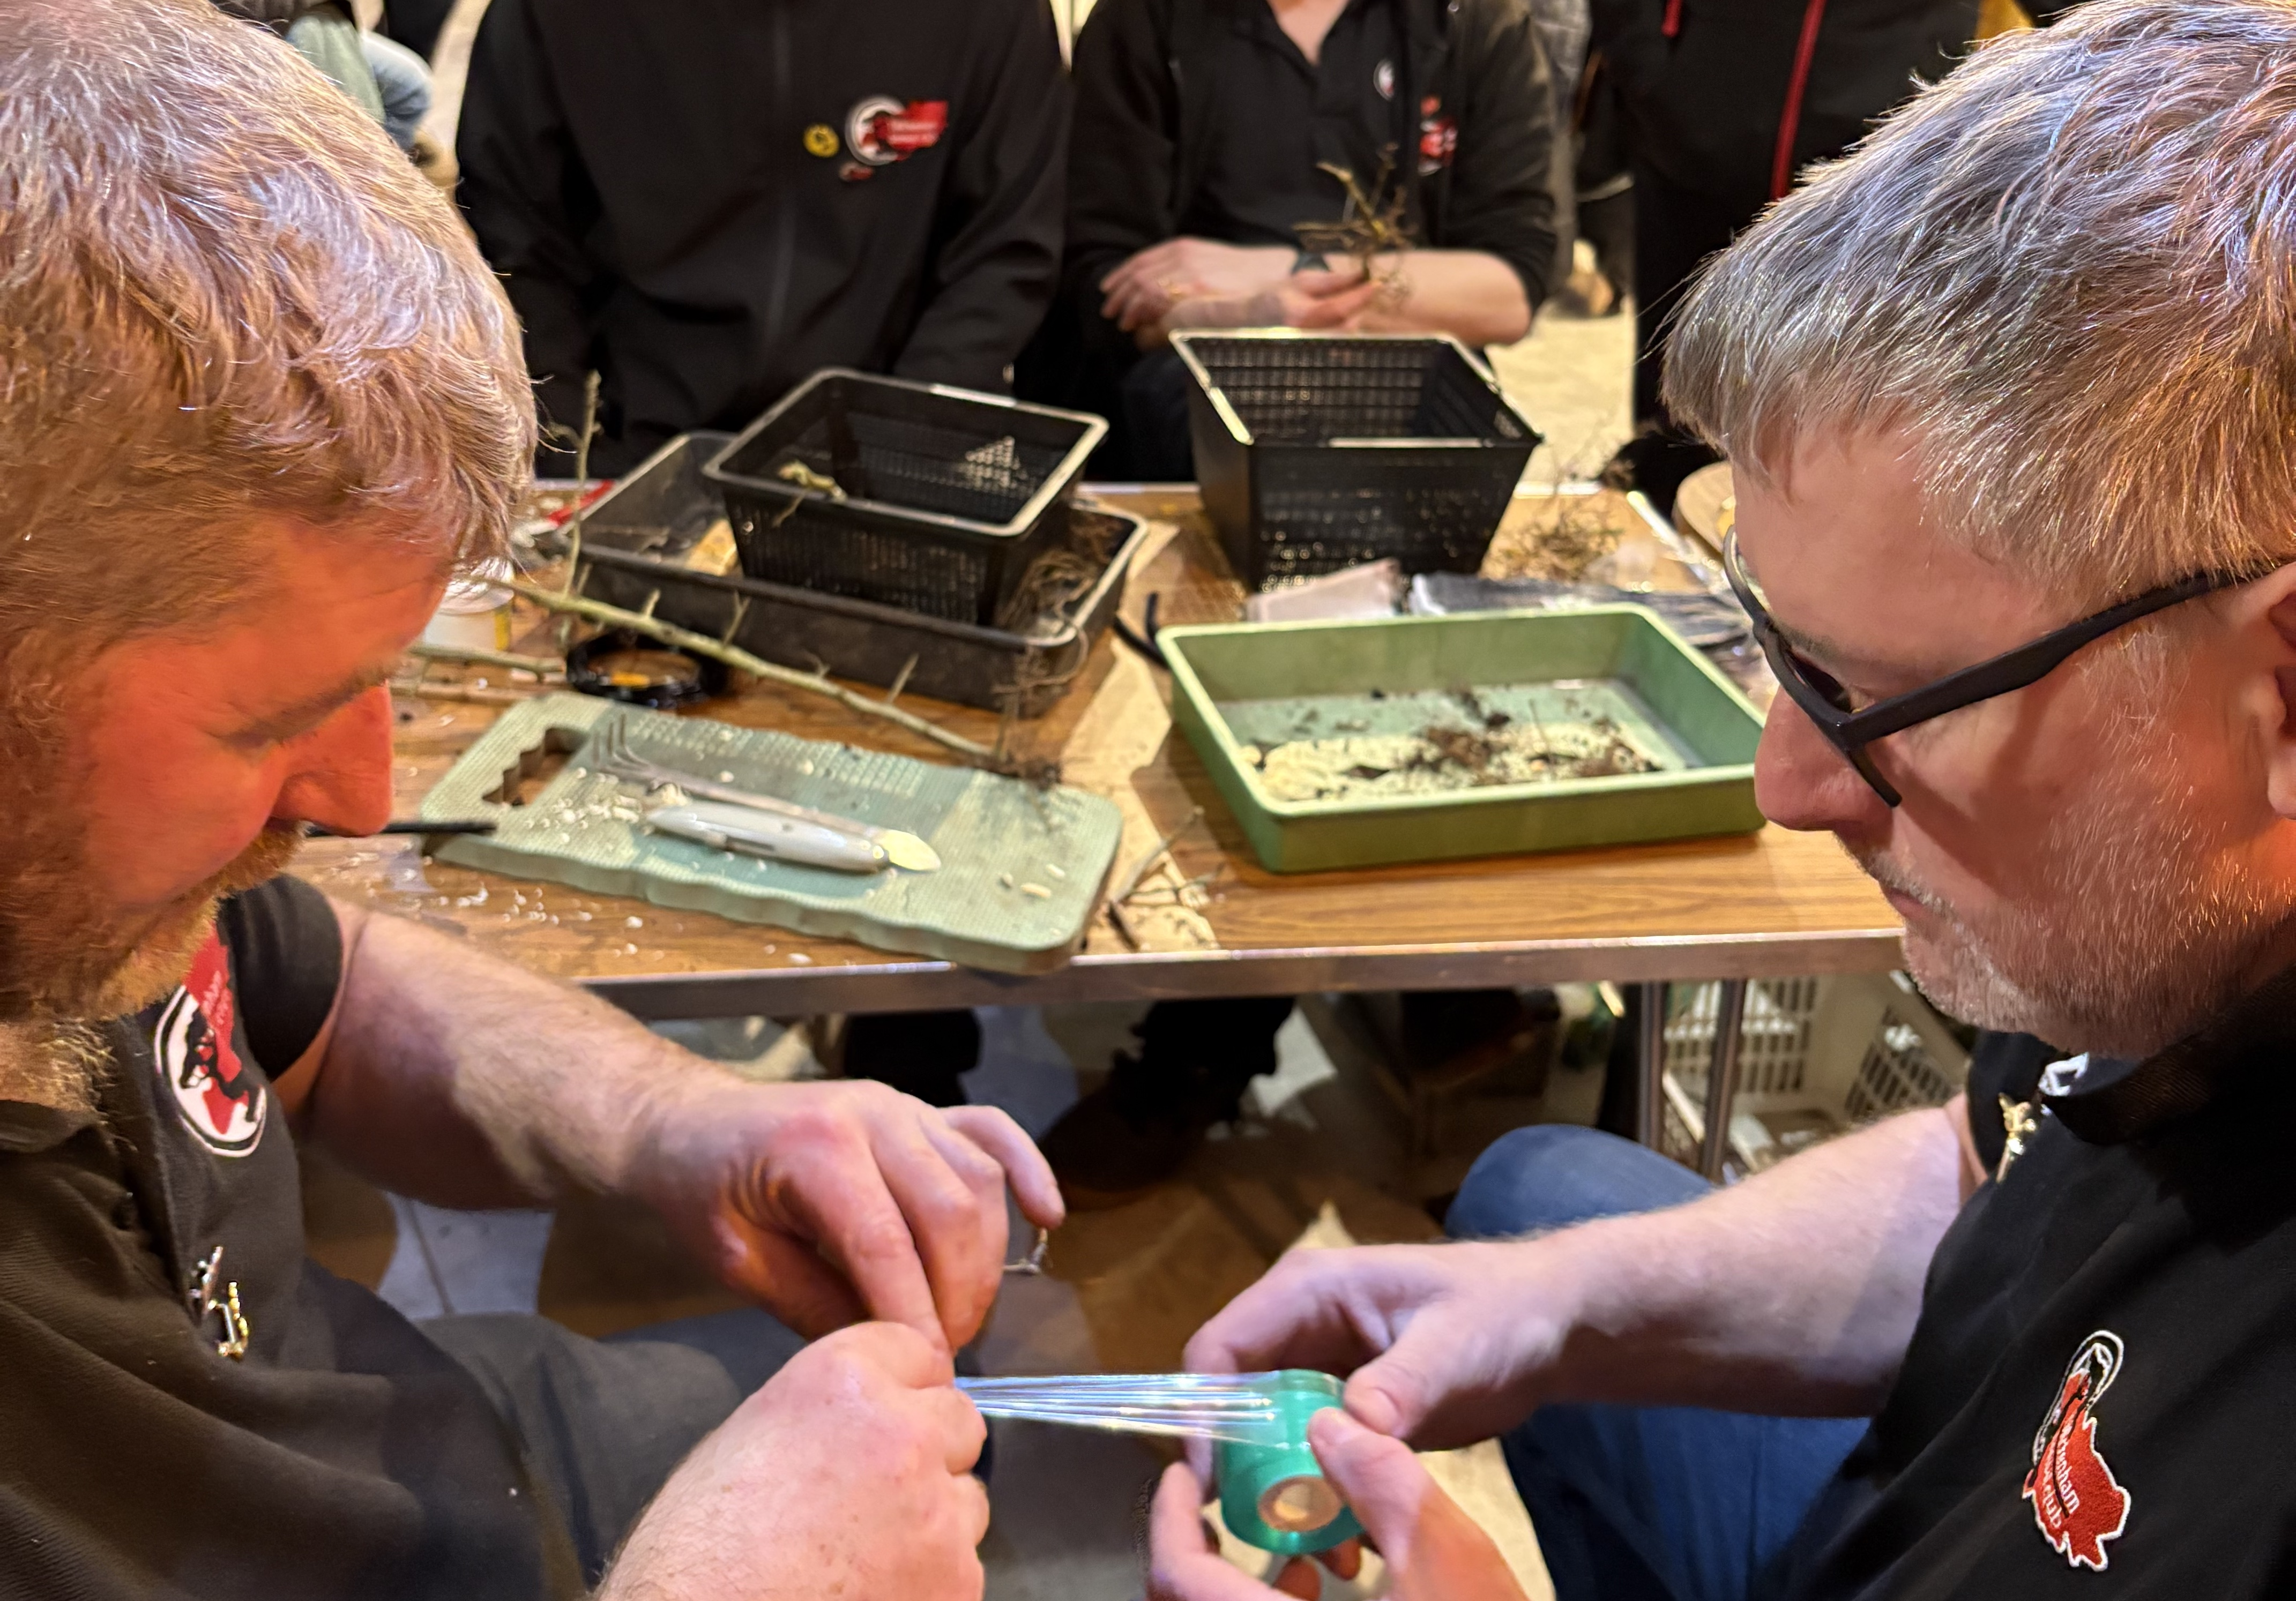
\includegraphics[width=1.0\columnwidth]{2025_02/res/grafting.jpg},%
    \centerline{\emph{Members gather around as Steve demonstrates grafting at the February meeting.}}%
]
\end{window}
\closearticle
\clearpage